
\documentclass[11pt]{article}
\usepackage{geometry}                % See geometry.pdf to learn the layout options. There are lots.
\geometry{letterpaper}                   % ... or a4paper or a5paper or ... 
%\geometry{landscape}                % Activate for for rotated page geometry
%\usepackage[parfill]{parskip}    % Activate to begin paragraphs with an empty line rather than an indent
\usepackage{../../doublespace}
\usepackage{../../algorithm,../../algorithmic}
\usepackage{graphicx}
\usepackage{amssymb}
\usepackage{epstopdf}
\usepackage{listings}

\DeclareGraphicsRule{.tif}{png}{.png}{`convert #1 `dirname #1`/`basename #1 .tif`.png}

\newtheorem{thm}{Theorem}[section]
\newtheorem{adef}[thm]{Definition}
\newtheorem{cor}[thm]{Corollary}
\newtheorem{lem}[thm]{Lemma}


\title{Quartz Renaissance Solutions on k-Means Estimators}
\author{Dan Beatty}
\begin{document}
\section{Introduction}

\section{Mathematical Description}


\begin{algorithm}
\caption{k-Means Estimation}
\label{alg:kMeans}
\begin{algorithmic}
	\REQUIRE $k$ the number of clusters
	\REQUIRE $S$ a set of samples arranged in $m \times n$ matrix \\
		where $m$ is the number of attributes, \\
		$n$ is the number of samples.
	\STATE Set means matrix $Q$ such that $Q$ is $m \times k$
	\STATE Select $k$ columns from $S$ at random and insert them into $Q$
	\REPEAT
		\STATE Create $Q'$ s.t. $Q = 0$ and $Q'$ is $m \times k$.
		\STATE Create row vector $\vec{r}$ so that $\vec{r}$ is $1 \times k$
		\FOR { each $\vec{s}_j \in S$, where $\vec{s}_j$ is the $j$th column of $S$}
			\STATE Measure distance w/ the columns in $Q$
			\STATE Identify the smallest distance column, $t$.
			\STATE Add $\vec{s}_j$ to $\vec{q'}_t$, and insert into $Q'$ at column $t$
			\STATE Increments $r_t$
		\ENDFOR
		\STATE Scale divide: $Q'$ with $\vec{r}$
		\STATE $\epsilon = |Q - Q'|$
		\STATE $Q \leftarrow Q'$
	\UNTIL {$\epsilon$ is satisfied}
	\ENSURE {$Q$}
\end{algorithmic}
\end{algorithm}


\begin{figure}[htbp] %  figure placement: here, top, bottom, or page
   \centering
   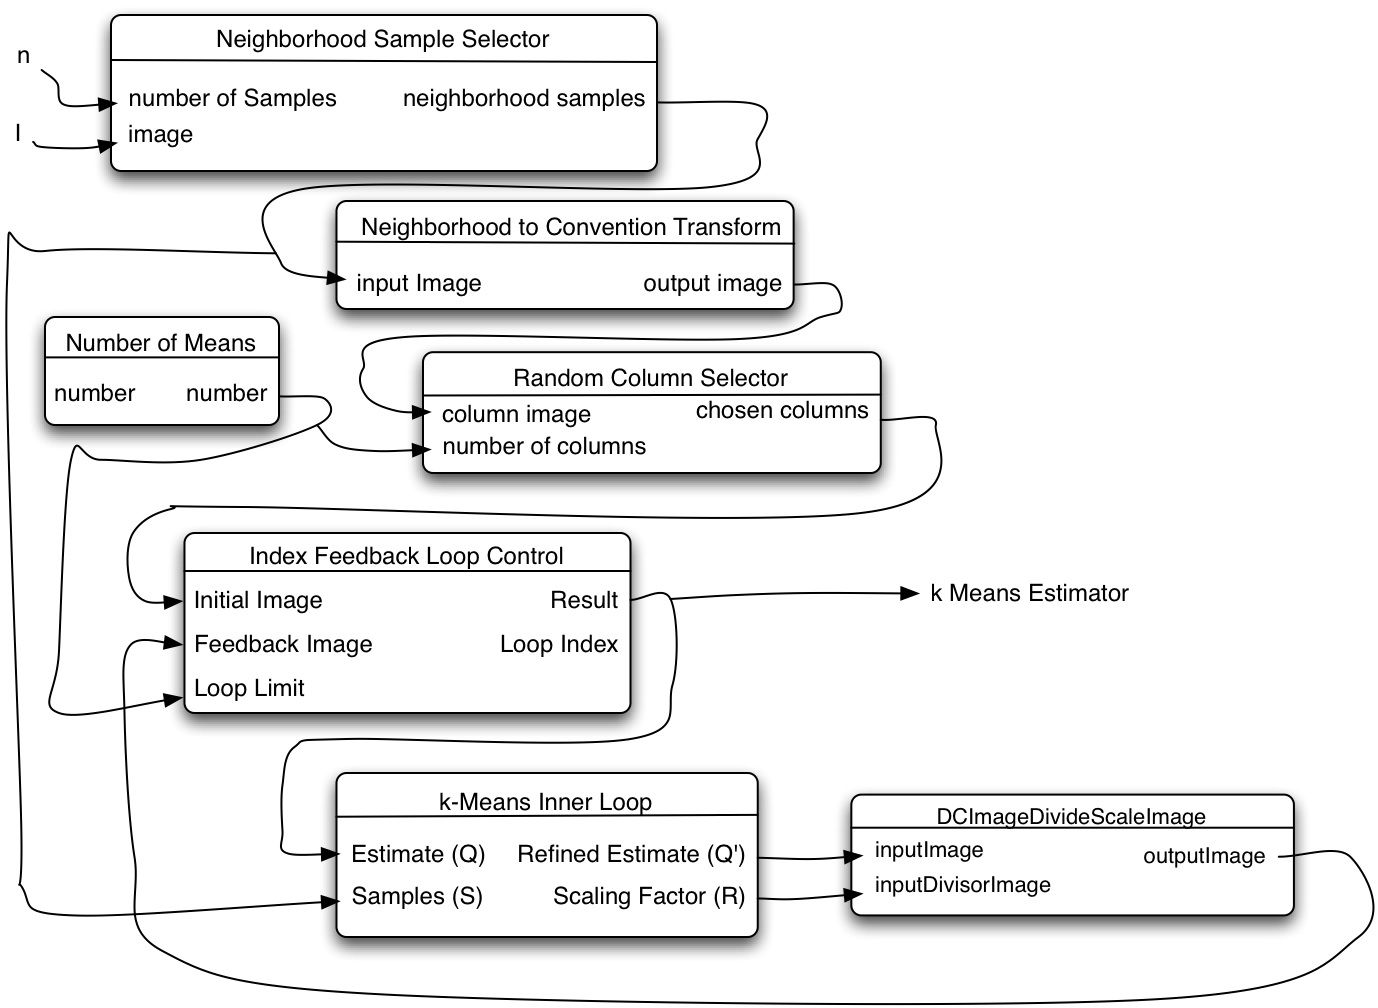
\includegraphics[width=5in]{kMeansOuterLoop.jpg} 
   \caption{k-Means Outer Loop}
   \label{kMeansOuterLoop}
\end{figure}



\begin{figure}[htbp] %  figure placement: here, top, bottom, or page
   \centering
   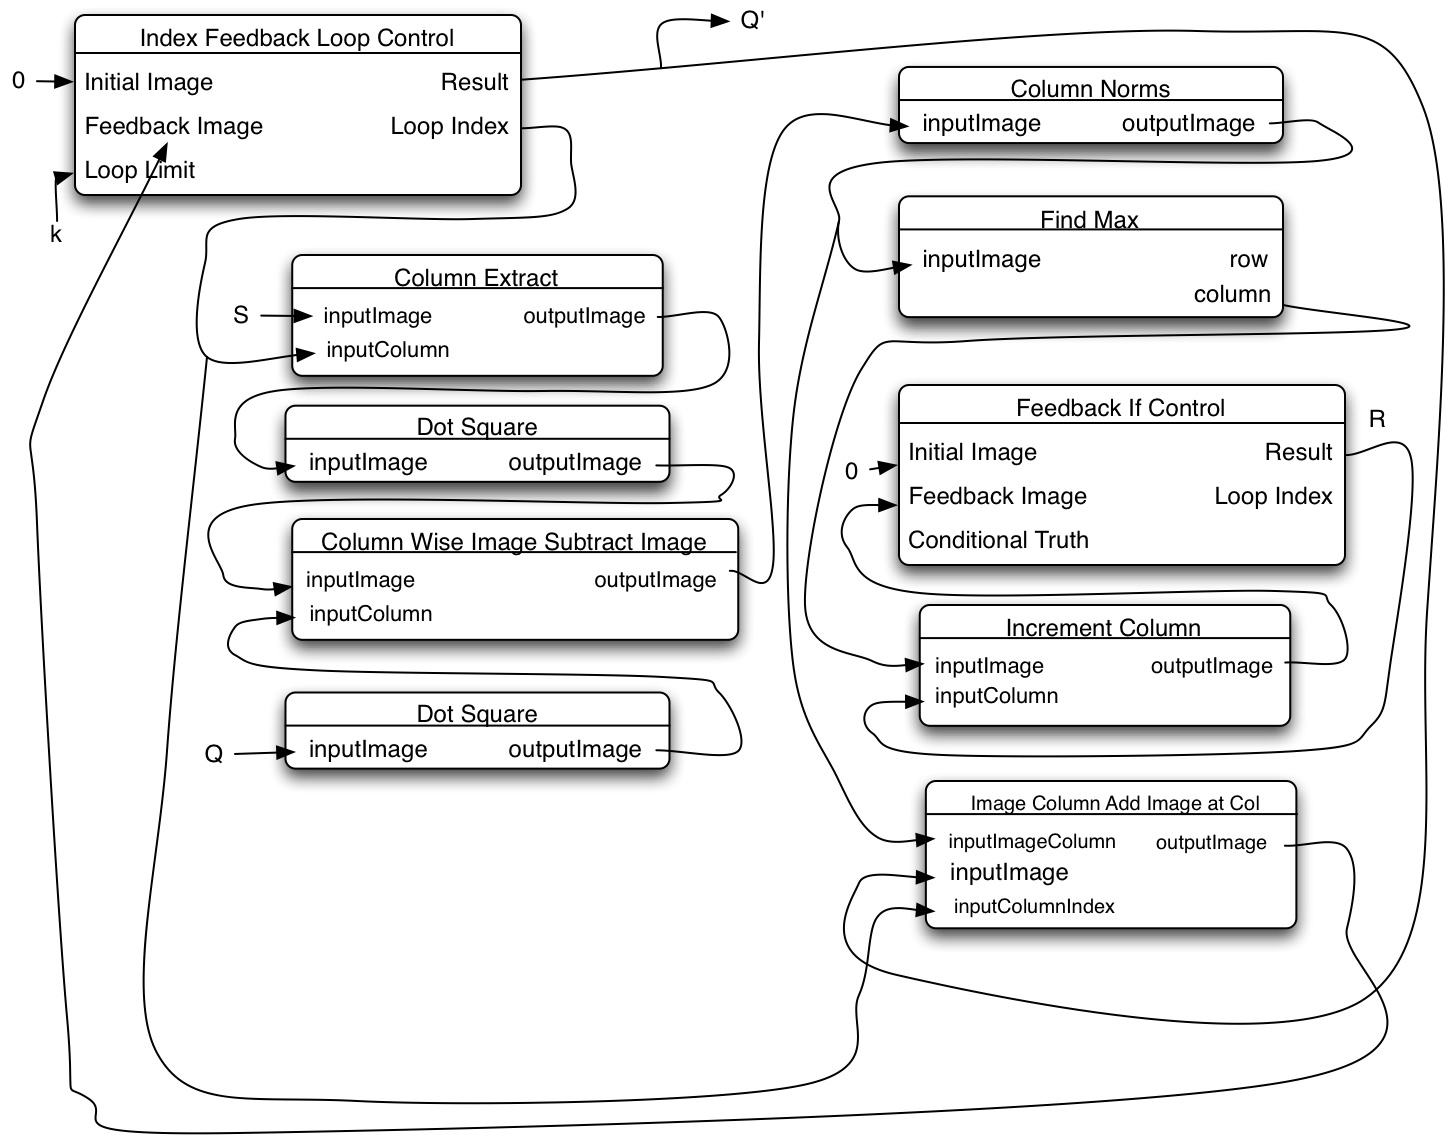
\includegraphics[width=6in]{kMeansInnerLoop.jpg} 
   \caption{k-Means Inner Loop}
   \label{kMeansOuterLoop}
\end{figure}

One key of the Loop Controller is the need to store a copy of the results image.  In the case of the Iterative Feedback Loop Control, that stored copy is used as the output after the loop has passed the maximum value.

\bibliography{../patternNotes.bib}
\bibliographystyle{abbrv}
\end{document}